\section{The waypoint system}
\label{sec:wayPointSystem}

\subsection{Concept}

To enable the drivers to see things in the world, we developed a system of 
objects that we call the waypoints. When a driver looks at it's vicinity, all
things in this area are collected and passed to the driver as waypoints. With
this concept, all objects in the world can be treated similarly.\\

\noindent The area that describes what the driver can see is implemented as the 
''driver view`` (\ref{sec:driverView}) and is based on the manner 
how humans view their environment. \\

\noindent To have an efficient filter for the waypoints we implemented a quad tree 
(\ref{sec:quadTree}).

\subsection{Types of waypoints}

We thought about the things that a driver would see when driving through a 
street that could have an effect on his behaviour. Such things could be

\begin{itemize}
\item Other vehicles (cars, bicycles, trucks,...)
\item Pedestrians
\item Road signs
\item Junctions
\item Pedestrian crossings
\item ...
\end{itemize}

For this project, we decided to implement only the waypoints for 
cars, junctions and speed signs, but the design should still be open for 
other waypoints in a later stage of the project. So we came up with following
class design:

\begin{figure}[htb]
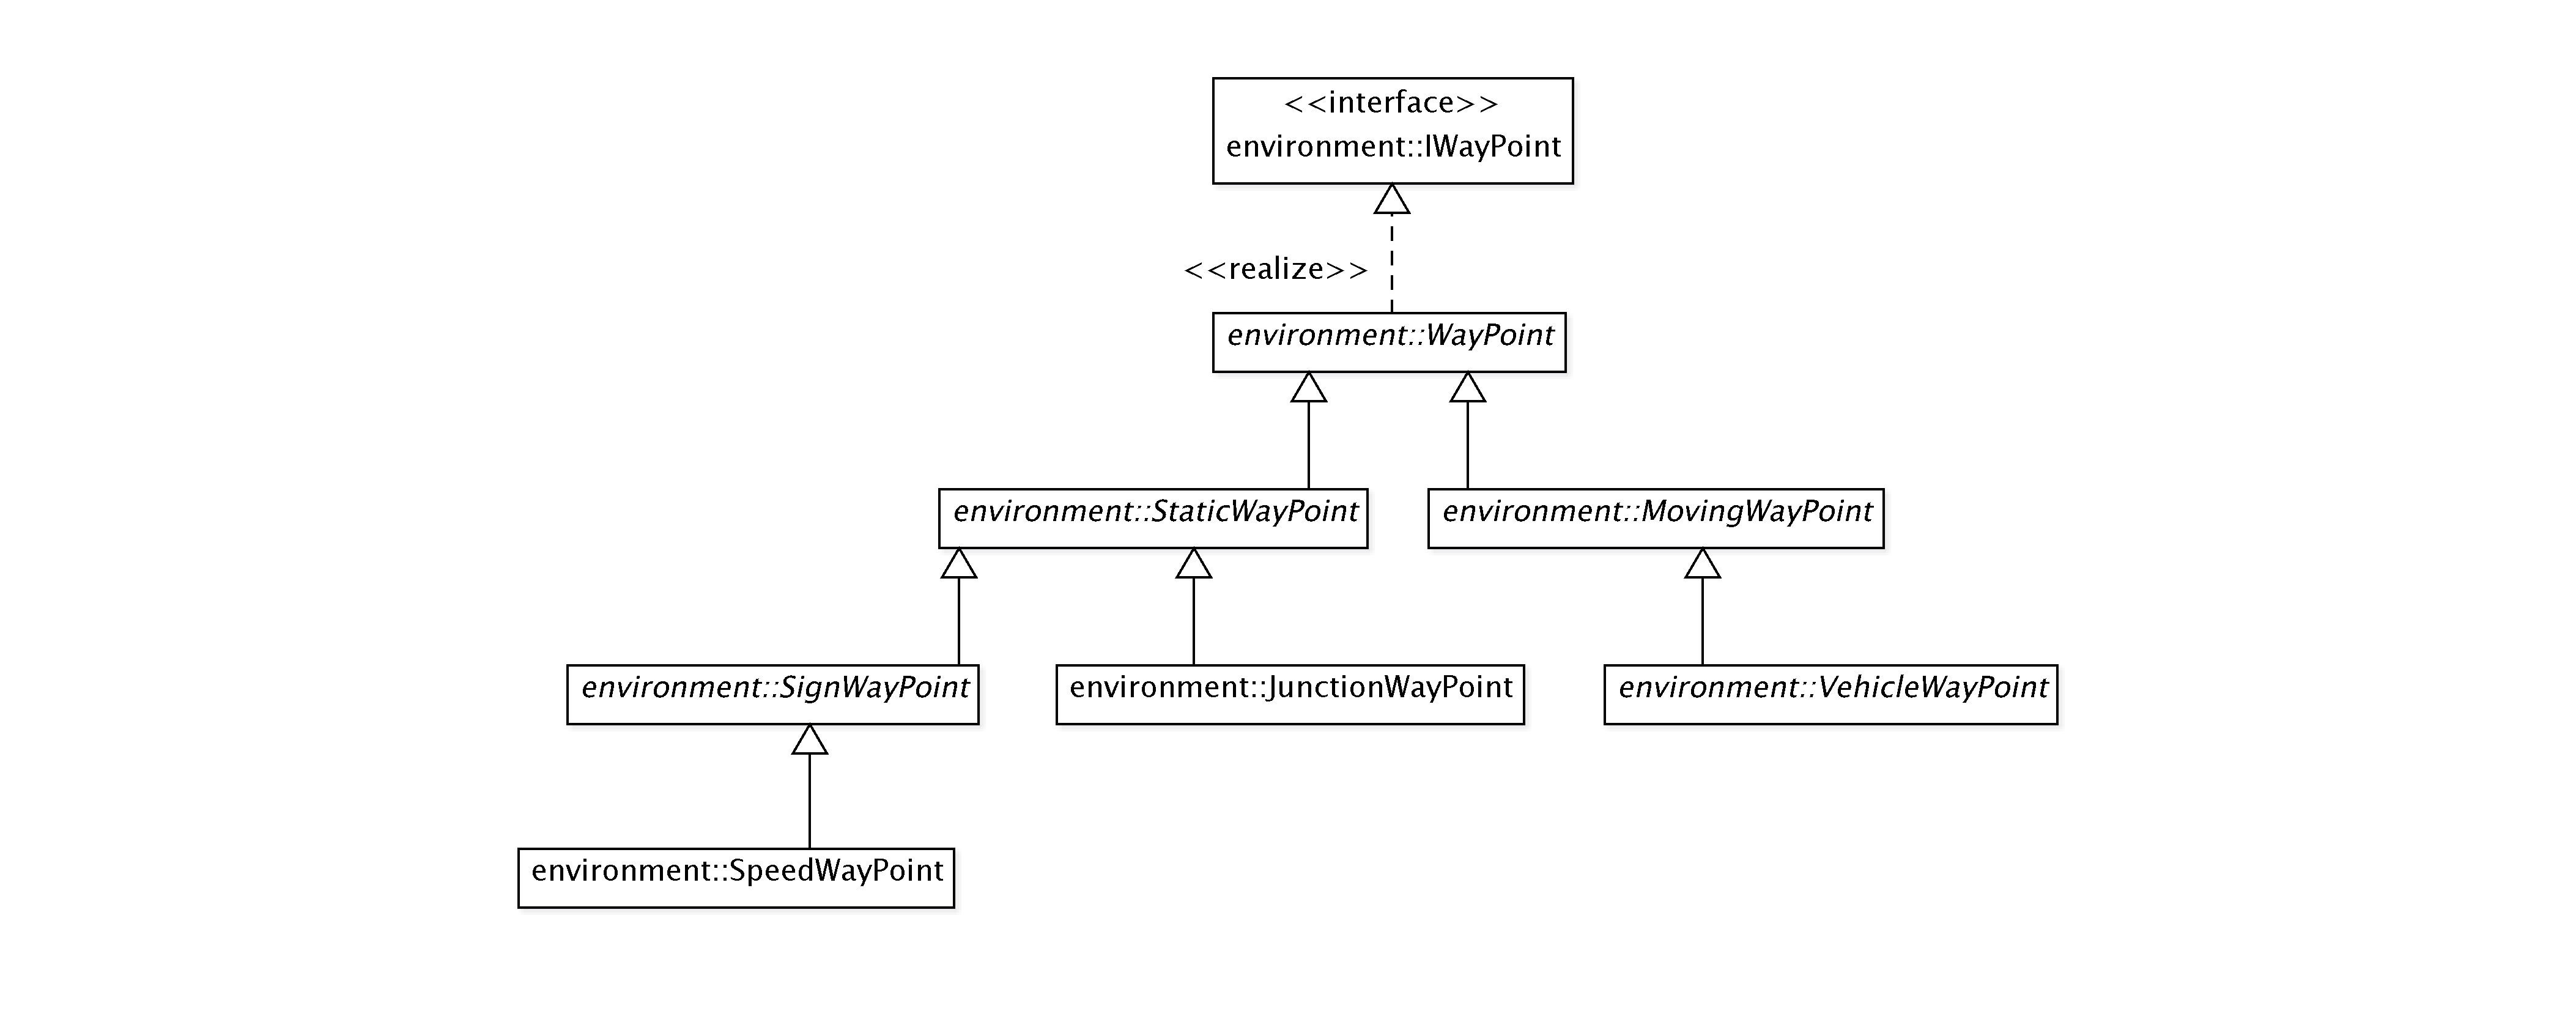
\includegraphics[width=\textwidth]{images/waypoints.png}
\caption{The class design of the waypoints}
\label{fig:waypoints}
\end{figure}

\noindent The implemented waypoints are described further below. \\

\subsubsection{Waypoint distance}
\label{sec:movingWPDistance}
A property that all waypoints have is a method to 
return the distance to another vehicle. To make it more realistic, some random 
error is added to this distance, since humans can only estimate distances.

\subsubsection{Static waypoints}

The static waypoints are those that will never be moved in the world.
They are given by the XML file that describes the world (\ref{sec:XML}).

\paragraph{Junction waypoints}
A junction waypoint describes a junction. It provides the information, in
which directions the driver can go. Junction waypoints are generated by the
junctions and placed on the lanes (\ref{sec:roadModel}) at the position of
80\% of the lane length.

\paragraph{Speed waypoints}
The speed waypoints are road signs that restrict the speed limit to a certain
value. To keep things simple, there is, unlike in the real world, no sign to 
abrogate the speed limit to the default value. \\

\subsubsection{Moving waypoints}

Some of the waypoints represent moving objects. Since we only have cars in this
project so far, only those waypoints are needed. \\

\paragraph{Car waypoints}
These waypoints represent other cars in the simulation. Each car generates its
waypoint and updates its position as the car moves.

\subsection{Waypoint finding}

The search for waypoints that a driver can see when driving on ordinary lanes 
is achieved in three steps:

\begin{itemize}
\item Filter with a quad tree
\item Filter with the driver view
\item Check the lanes
\end{itemize}

The waypoint finding around junctions is slightly different, see section 
\ref{sec:junctionWPfinding}.

\subsubsection{The quad tree}
\label{sec:quadTree}

To be able to locate the waypoints in a certain area quickly, they are
organized in a quad tree. The quad tree basically divides the world
into rectangles as shown in figure \ref{fig:quadTree} to a certain
depth, which are nodes in the tree. The depth defines the resolution
of the tree, and depending on the depth the nodes cover each an area
in the world. The nodes are created only if there are waypoints their
area. They can contain more than one waypoint, since there can be more
than one waypoint in an area.\\

\begin{figure}[H]
\begin{center}
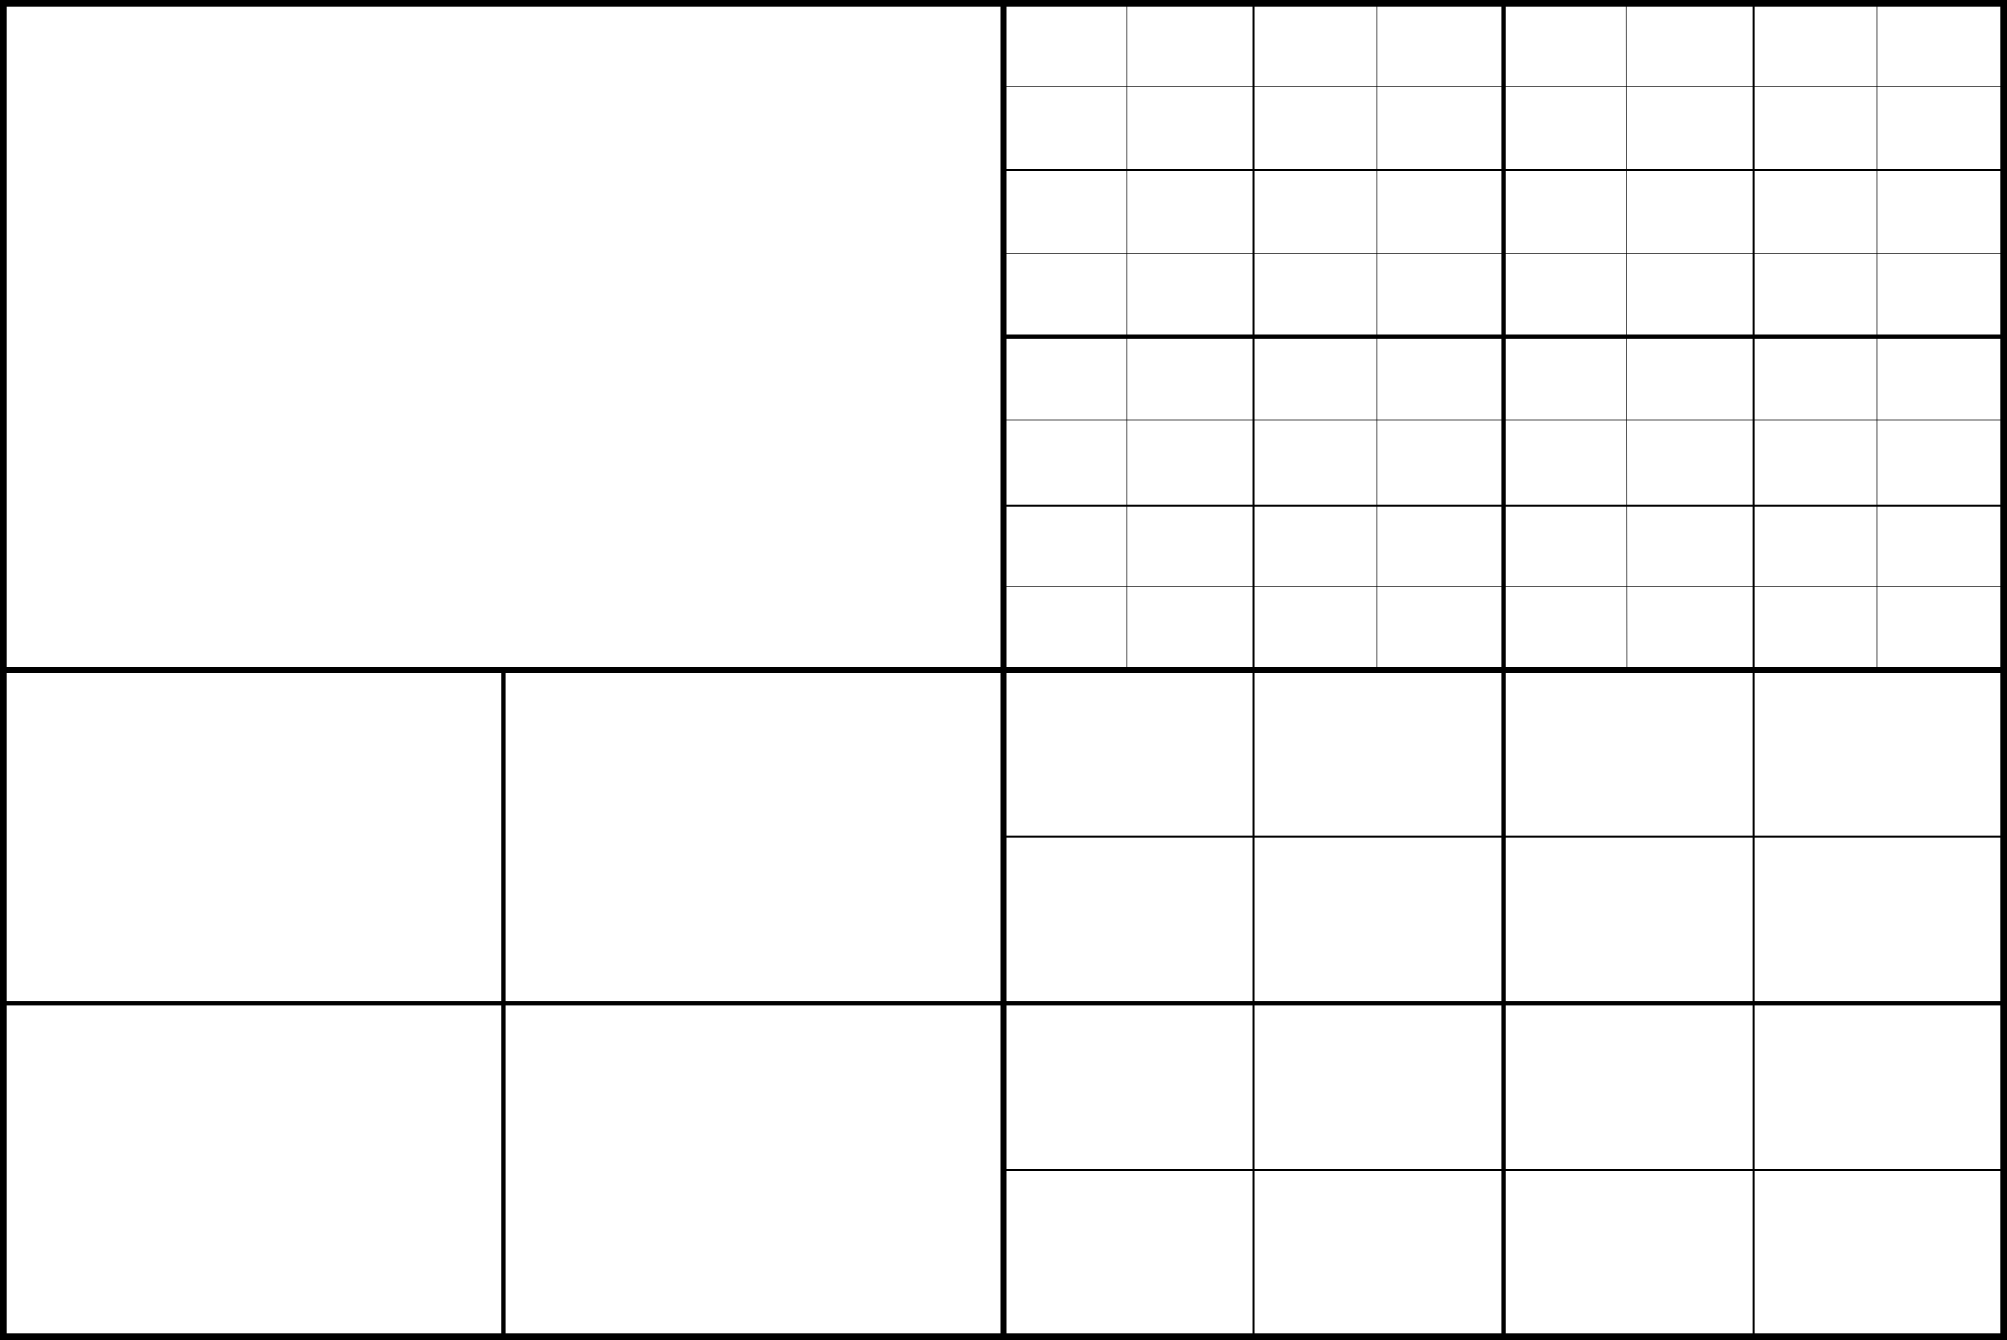
\includegraphics[scale=0.5]{images/quadtree.png}
\end{center}
\caption{The fragmentation of the quad tree with different depths up to depth 
4 in the top right corner}
\label{fig:quadTree}
\end{figure}

\noindent With this implementation, all the nodes in the vicinity of the
vehicle can be found with O(d) where d is the depth of the three. Since
the quad tree is based on rectangles, the results have to be filtered
further to determine if the located waypoints really lie in the driver
view, which is explained in the next chapter.\\

\noindent The rectangles to use for the search are calculated from the
driver view. Rectangles that enclose the whole driver view are taken
for the search.

\noindent Figure \ref{fig:quadTreeClasses} shows the composition of the
quad tree classes.

\begin{figure}[H]
\begin{center}
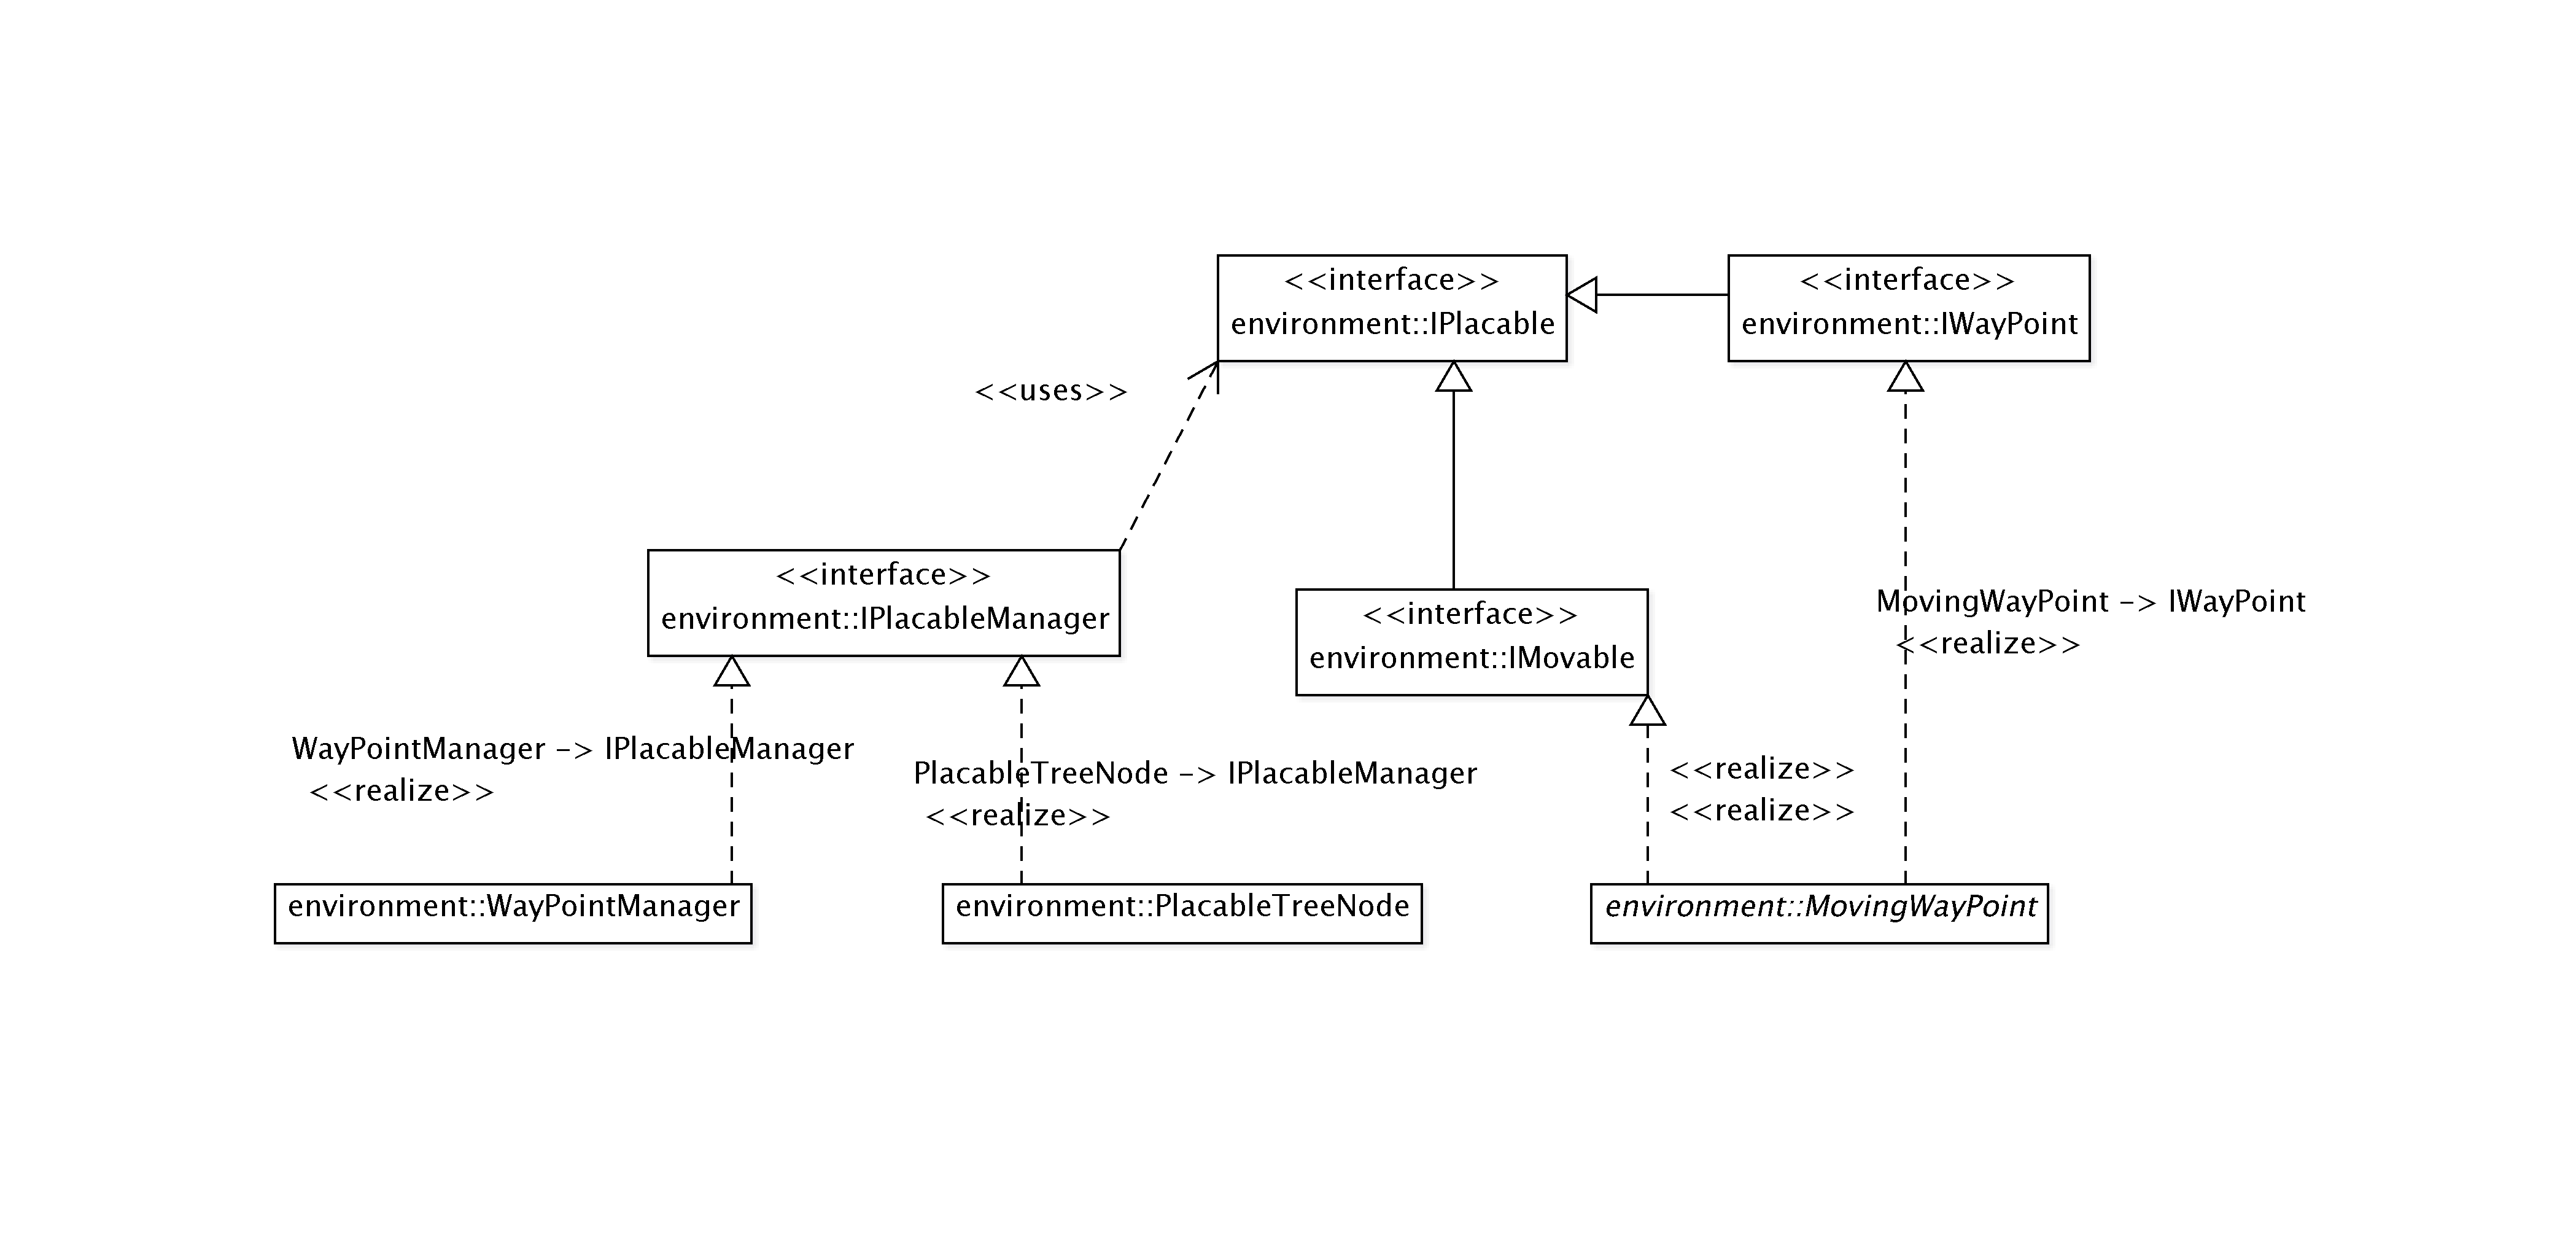
\includegraphics[width=\textwidth]{images/waypointsmanager.png}
\end{center}
\caption{The quad tree classes}
\label{fig:quadTreeClasses}
\end{figure}

\subsubsection{The driver view}
\label{sec:driverView}

\paragraph{Description}

The driver view describes the area wherein the driver can see other objects in
the world. It is described by following parameters:

\begin{itemize}
\item \textbf{Direction} The direction the driver looks
\item \textbf{Position} The position of the driver view 
\item \textbf{Angle} The angle of the visual field
\item \textbf{Distance} The distance that the driver can see
\end{itemize}

\noindent Drugs can be applied to these parameters. They can have a certain effect
on each of the parameters. \\

\noindent With this system of parameters we tried to make the driver view as 
realistic as possible. At first we had a driver view shaped as a triangle, 
which was based on the human field of view.
Figure \ref{fig:driverView} depicts this driver view.

\begin{figure}[H]
\begin{center}
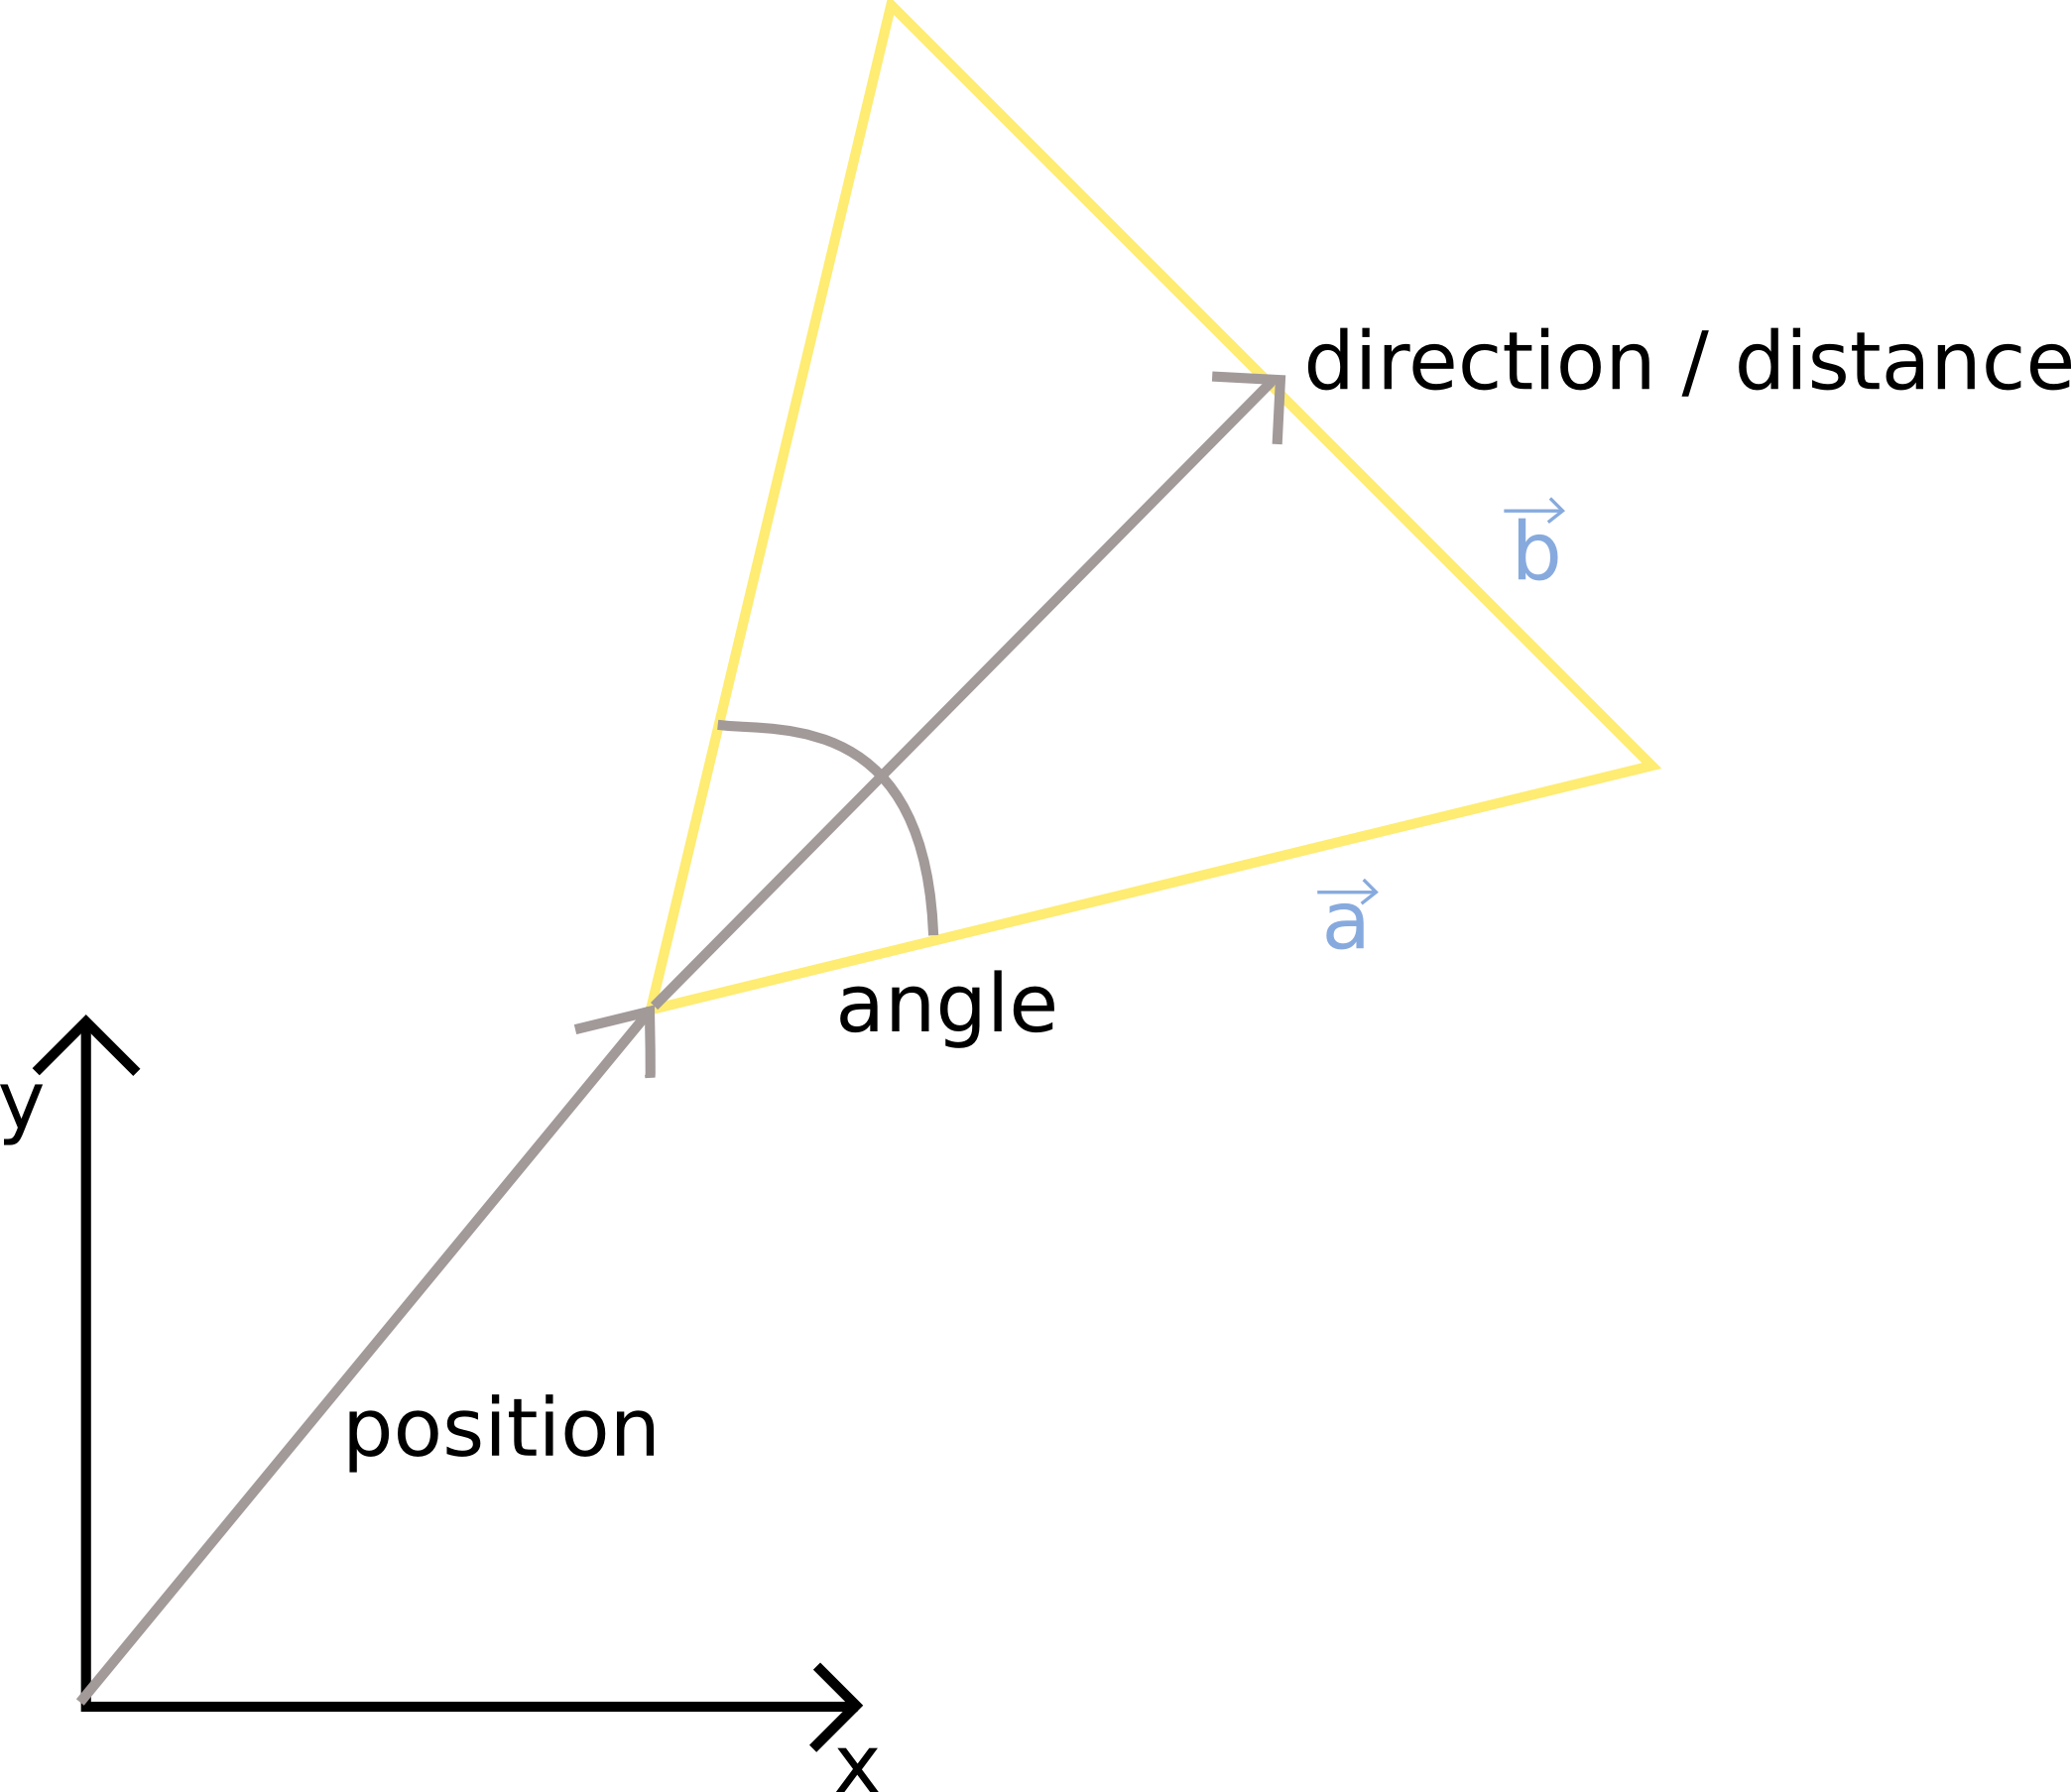
\includegraphics[scale=0.4]{images/driverview.png}
\end{center}
\caption{The first driver view}
\label{fig:driverView}
\end{figure}

\noindent During the development we realized that, although this driver
view worked well for straight lanes, it posed a few problems with
situations like curves and junctions.  In these situation the driver
should have the possibility to look around. Instead of enabling him to
do so we implemented a new version of the driver view that enables him
to see more in the world. It is shaped like this:

\begin{figure}[H]
\begin{center}
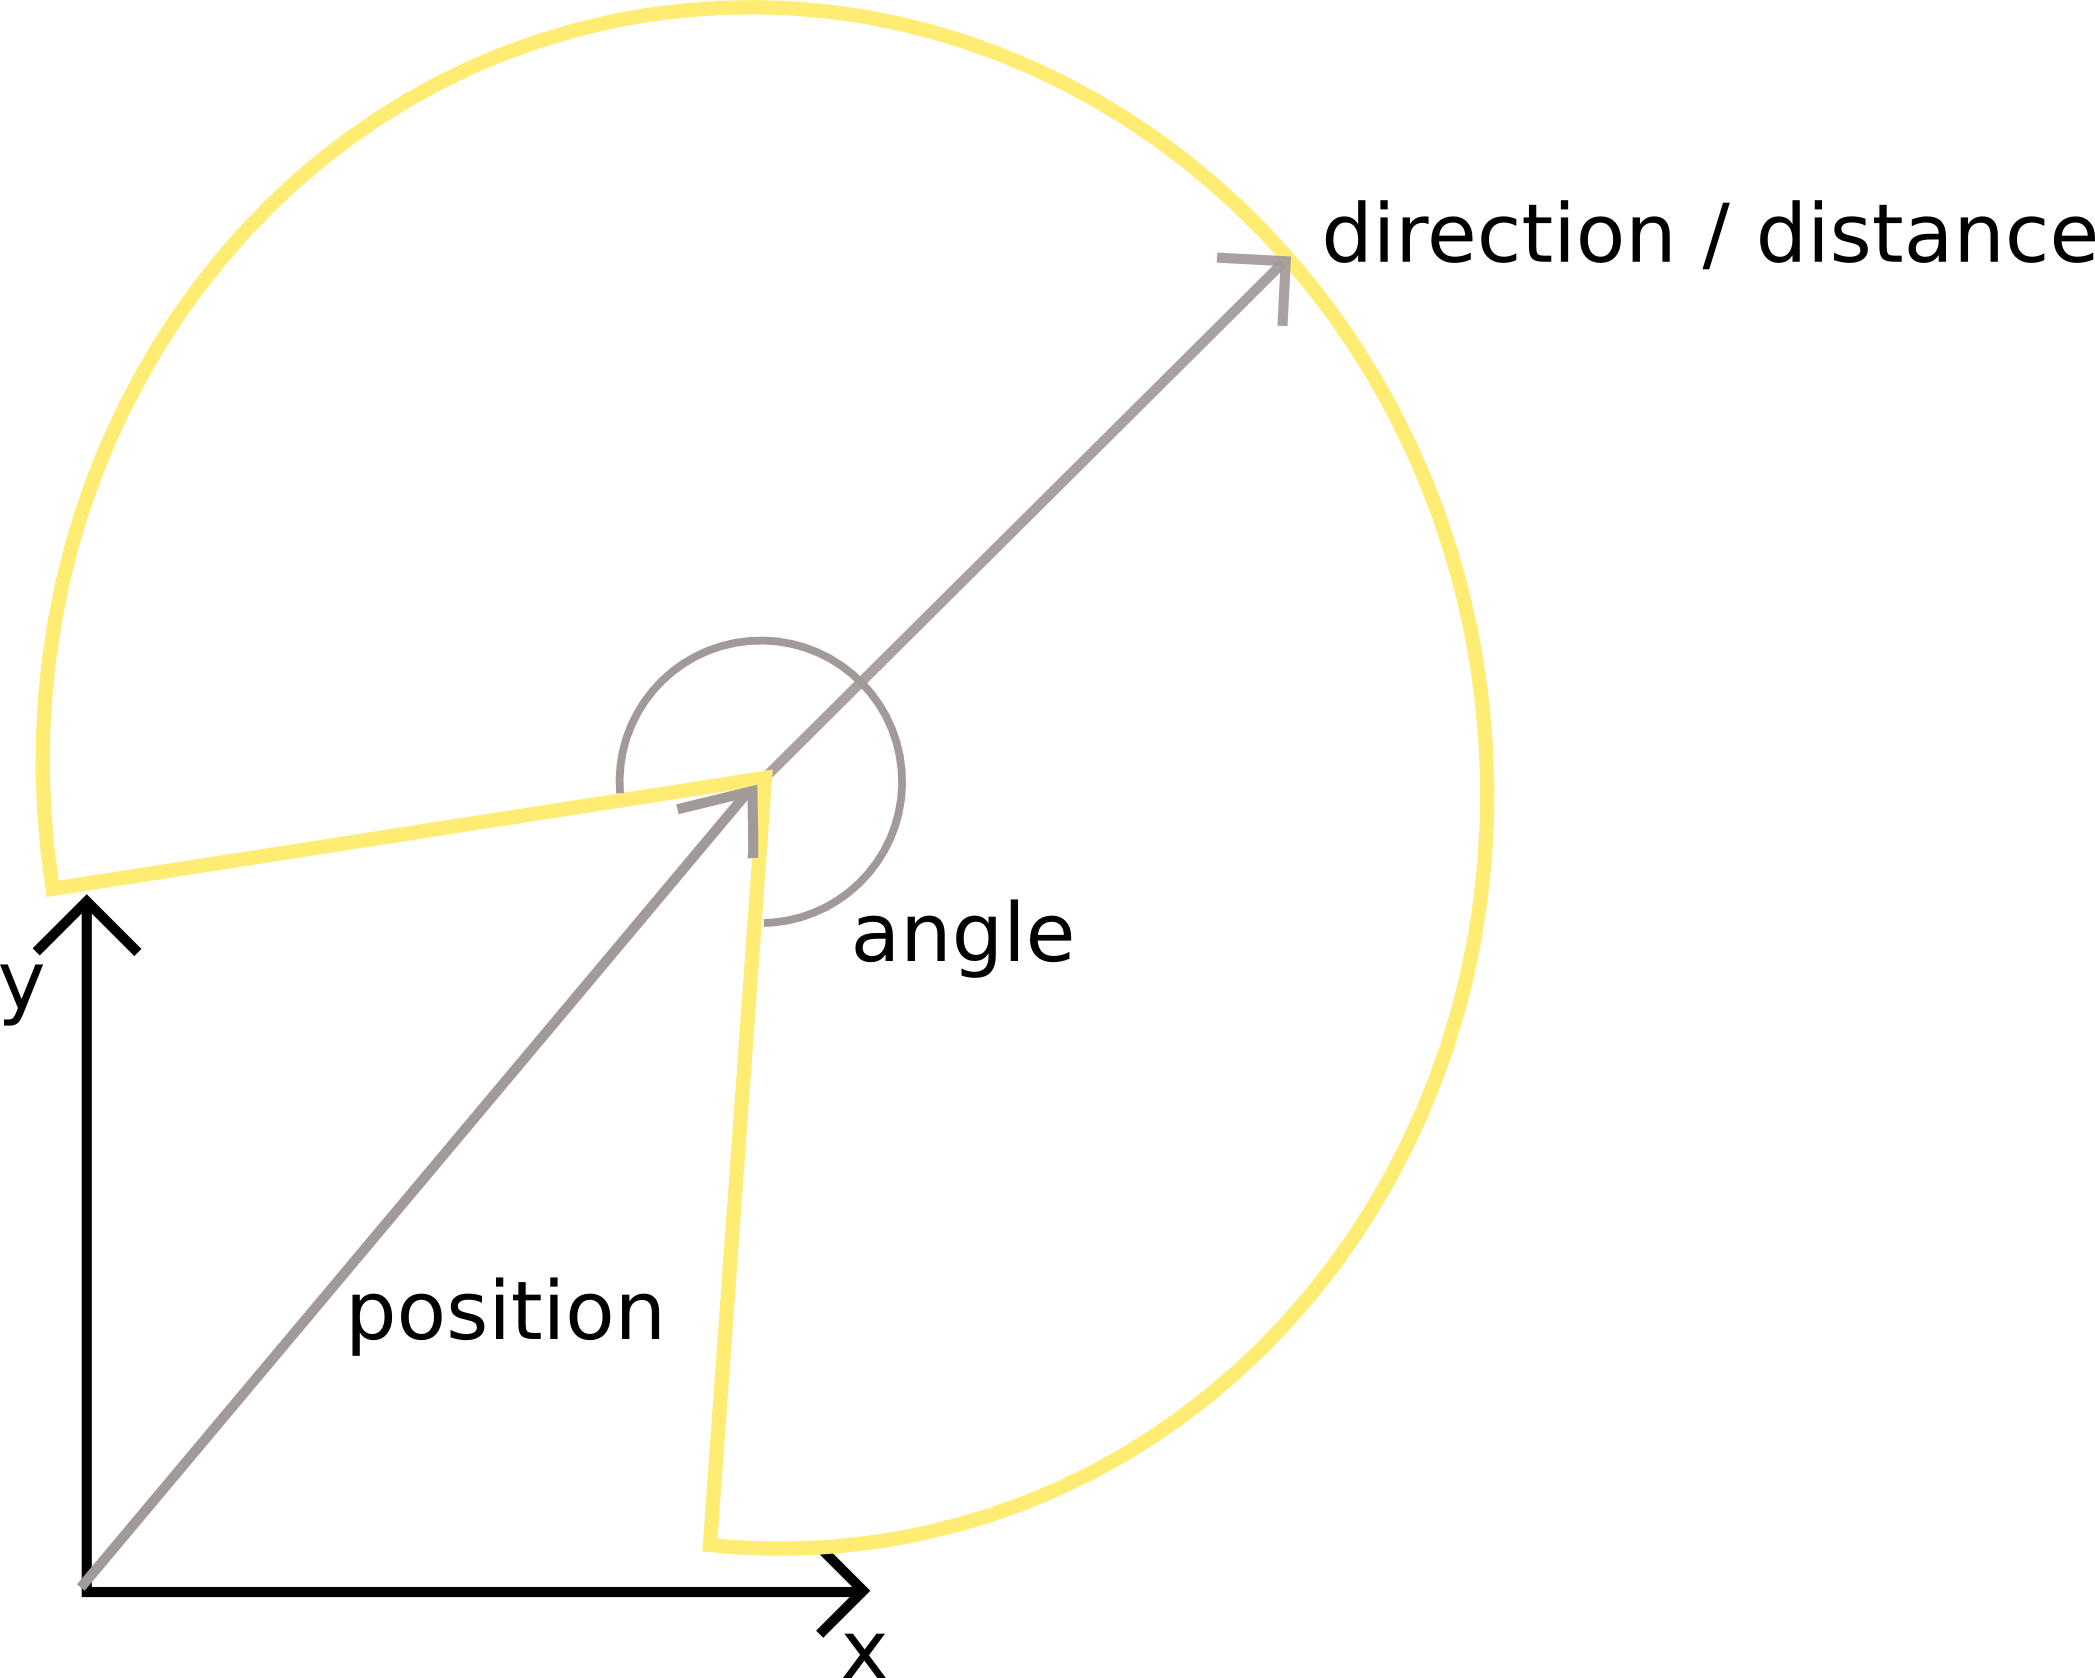
\includegraphics[scale=0.4]{images/driverviewcircled.png}
\end{center}
\caption{The new driver view}
\label{fig:driverViewCircled}
\end{figure}

\noindent With this shape the driver is able to look around the curves
and also see things on a crossing lane. Thanks to an interface for the
driver view we could just replace the triangular driver view with the new,
round one without having to change the other parts of the code.

\paragraph{The filtering}

After the quad tree (\ref{sec:quadTree}) has completed its search, the
located waypoints are filtered further to take account of the angled
driver view instead of using just a rectangle. \\

The algorithm to determine whether a waypoint lies in the triangular
driver view, is based on a linear equation which we implemented globally
in the vector class (\ref{sec:linearCombination}). If following
constraints are fulfilled, the waypoint lies in the driver view
triangle: \\

$ \lambda, \mu \in ]0, 1]$ \\

$ \frac{\lambda * \left| \vec{b} \right| }{\mu * \left| \vec{a} \right|} \leq 
\frac{\left| \vec{b} \right|}{\left| \vec{a} \right|}$ \\

\noindent Where $\lambda$ and $\mu$ are the components of the linear combination \\

$ \lambda * \vec{a} + \mu * \vec{b} $ \\

The algorithm for the Pacman-shaped waypoint is simpler. Assuming
$\vec{v}$ is the position vector of the waypoint, $\vec{p}$ the
one of the driver view and $\alpha$ is the angle of $\left | \vec{v} -
\vec{p}\right|$ to the x-axis, following constraints have to be fulfilled
(here the distance is the radius of the circle): \\

$ \left| \vec{v} - \vec{p} \right| \leq \text{distance}$  \\

$ -\frac{\text{angle}}{2} < \alpha < \frac{\text{angle}}{2} $


\subsubsection{Lane check}

At the last step of waypoint finding, the waypoints are checked with the
lane queue of the vehicle (\ref{sec:laneChanges}). If the waypoint is not
on any of the lanes in the vehicle's queue, it is dropped, since it doesn't
concern the driver. An example of such a waypoint is a vehicle on the lane
that goes in the opposite direction of the road.


\subsection{Junction waypoint finding}
\label{sec:junctionWPfinding}

TODO: document this



